\documentclass{standalone}
\usepackage{tikz}
\usetikzlibrary{patterns, positioning}


\begin{document}
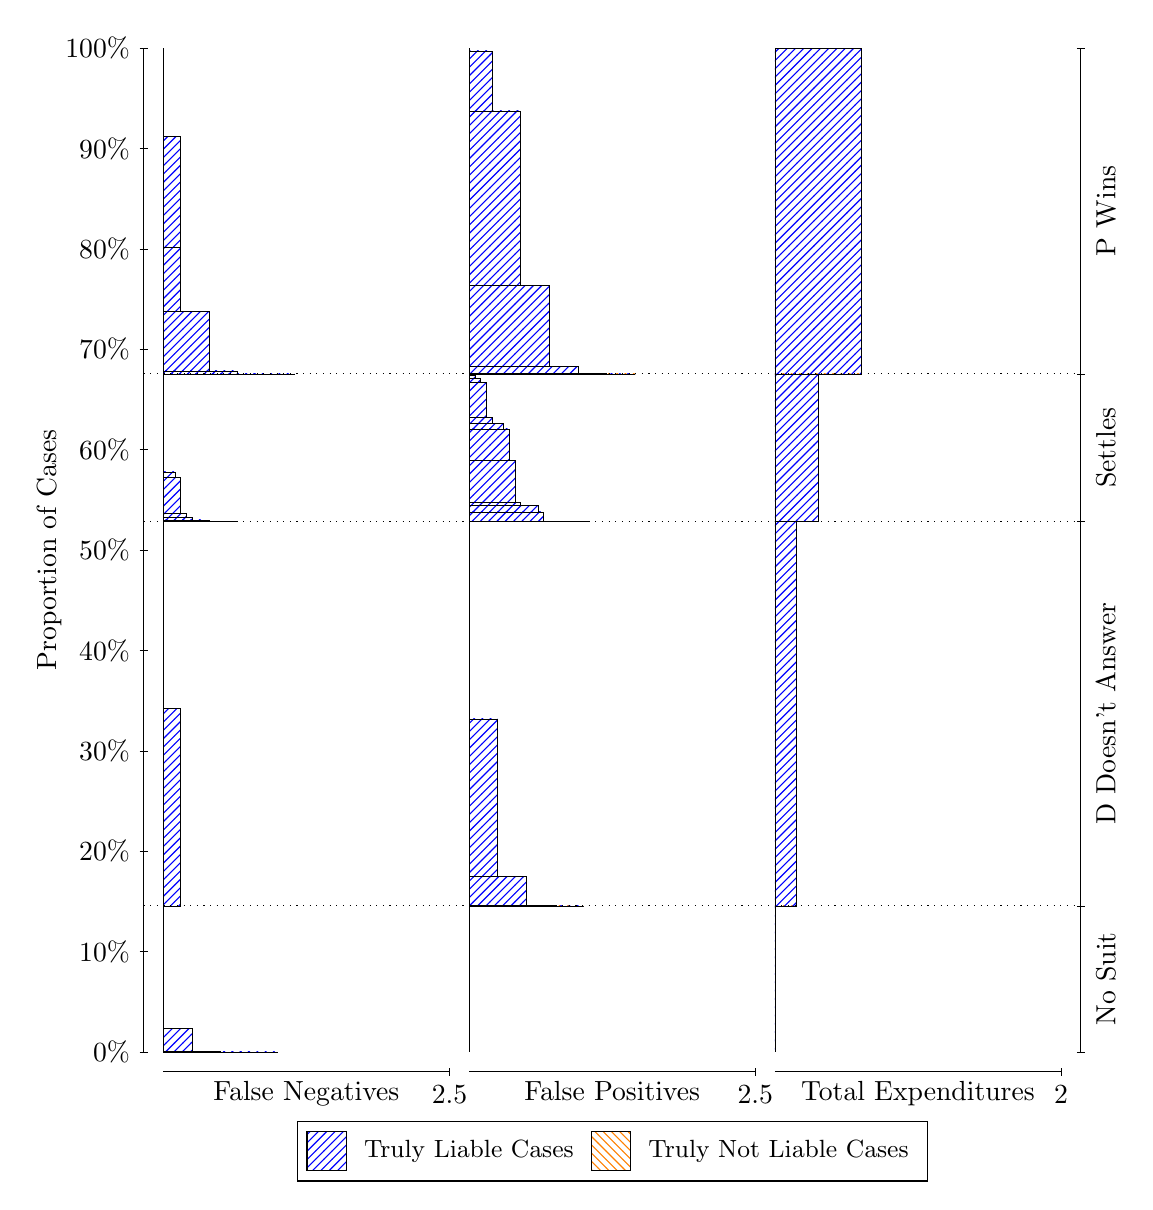
\begin{tikzpicture}
\draw[black, very thin] (1.5,1.75) -- (1.5,14.5);
\node[rotate=90, text=black, anchor=center] at (0.3, 8.125) {Proportion of Cases};
\draw[black, very thin] (1.45,1.75) -- (1.55,1.75);
\node[text=black, anchor=east] at (1.45, 1.75) {0\%};
\draw[black, very thin] (1.45,3.025) -- (1.55,3.025);
\node[text=black, anchor=east] at (1.45, 3.025) {10\%};
\draw[black, very thin] (1.45,4.3) -- (1.55,4.3);
\node[text=black, anchor=east] at (1.45, 4.3) {20\%};
\draw[black, very thin] (1.45,5.575) -- (1.55,5.575);
\node[text=black, anchor=east] at (1.45, 5.575) {30\%};
\draw[black, very thin] (1.45,6.85) -- (1.55,6.85);
\node[text=black, anchor=east] at (1.45, 6.85) {40\%};
\draw[black, very thin] (1.45,8.125) -- (1.55,8.125);
\node[text=black, anchor=east] at (1.45, 8.125) {50\%};
\draw[black, very thin] (1.45,9.4) -- (1.55,9.4);
\node[text=black, anchor=east] at (1.45, 9.4) {60\%};
\draw[black, very thin] (1.45,10.675) -- (1.55,10.675);
\node[text=black, anchor=east] at (1.45, 10.675) {70\%};
\draw[black, very thin] (1.45,11.95) -- (1.55,11.95);
\node[text=black, anchor=east] at (1.45, 11.95) {80\%};
\draw[black, very thin] (1.45,13.225) -- (1.55,13.225);
\node[text=black, anchor=east] at (1.45, 13.225) {90\%};
\draw[black, very thin] (1.45,14.5) -- (1.55,14.5);
\node[text=black, anchor=east] at (1.45, 14.5) {100\%};

\draw[black, very thin] (13.4,1.75) -- (13.4,14.5);
\draw[black, very thin] (13.35,1.75) -- (13.45,1.75);
\node[anchor=west] at (13.35, 1.75) {};
\draw[black, very thin] (13.35,3.6057) -- (13.45,3.6057);
\node[anchor=west] at (13.35, 3.6057) {};
\draw[black, very thin] (13.35,8.4872) -- (13.45,8.4872);
\node[anchor=west] at (13.35, 8.4872) {};
\draw[black, very thin] (13.35,10.363) -- (13.45,10.363);
\node[anchor=west] at (13.35, 10.363) {};
\draw[black, very thin] (13.35,14.5) -- (13.45,14.5);
\node[anchor=west] at (13.35, 14.5) {};

\draw[black, very thin, pattern color=blue, pattern=north east lines] (1.75,1.75) rectangle (3.2033,1.75);
\draw[black, very thin, pattern color=blue, pattern=north east lines] (1.75,1.75) rectangle (2.84,1.75);
\draw[black, very thin, pattern color=blue, pattern=north east lines] (1.75,1.75) rectangle (2.4767,1.7526);
\draw[black, very thin, pattern color=blue, pattern=north east lines] (1.75,1.7526) rectangle (2.1133,2.0538);
\draw[black, very thin, pattern color=orange, pattern=north west lines] (1.75,2.0538) rectangle (1.75,2.0538);
\draw[black, very thin, pattern color=blue, pattern=north east lines] (1.75,2.0538) rectangle (1.75,3.6057);
\draw[black, very thin, pattern color=blue, pattern=north east lines] (1.75,3.6057) rectangle (1.968,6.1122);
\draw[black, very thin, pattern color=orange, pattern=north west lines] (1.75,6.1122) rectangle (1.75,6.1122);
\draw[black, very thin, pattern color=blue, pattern=north east lines] (1.75,6.1122) rectangle (1.75,8.4872);
\draw[black, very thin, pattern color=blue, pattern=north east lines] (1.75,8.4872) rectangle (2.6947,8.4872);
\draw[black, very thin, pattern color=blue, pattern=north east lines] (1.75,8.4872) rectangle (2.404,8.4873);
\draw[black, very thin, pattern color=blue, pattern=north east lines] (1.75,8.4873) rectangle (2.3313,8.5034);
\draw[black, very thin, pattern color=blue, pattern=north east lines] (1.75,8.5034) rectangle (2.2587,8.5073);
\draw[black, very thin, pattern color=blue, pattern=north east lines] (1.75,8.5073) rectangle (2.1133,8.5427);
\draw[black, very thin, pattern color=blue, pattern=north east lines] (1.75,8.5427) rectangle (2.0407,8.5942);
\draw[black, very thin, pattern color=blue, pattern=north east lines] (1.75,8.5942) rectangle (1.968,9.0447);
\draw[black, very thin, pattern color=blue, pattern=north east lines] (1.75,9.0447) rectangle (1.8953,9.1183);
\draw[black, very thin, pattern color=orange, pattern=north west lines] (1.75,9.1183) rectangle (1.75,9.1183);
\draw[black, very thin, pattern color=blue, pattern=north east lines] (1.75,9.1183) rectangle (1.75,10.363);
\draw[black, very thin, pattern color=blue, pattern=north east lines] (1.75,10.363) rectangle (3.4213,10.363);
\draw[black, very thin, pattern color=blue, pattern=north east lines] (1.75,10.363) rectangle (3.058,10.363);
\draw[black, very thin, pattern color=blue, pattern=north east lines] (1.75,10.363) rectangle (2.6947,10.4);
\draw[black, very thin, pattern color=blue, pattern=north east lines] (1.75,10.4) rectangle (2.3313,11.16);
\draw[black, very thin, pattern color=blue, pattern=north east lines] (1.75,11.16) rectangle (1.968,11.973);
\draw[black, very thin, pattern color=blue, pattern=north east lines] (1.75,11.973) rectangle (1.968,13.378);
\draw[black, very thin, pattern color=orange, pattern=north west lines] (1.75,13.378) rectangle (1.75,13.378);
\draw[black, very thin, pattern color=blue, pattern=north east lines] (1.75,13.378) rectangle (1.75,14.5);
\draw[black, very thin, pattern color=orange, pattern=north west lines] (5.6333,1.75) rectangle (5.6333,1.75);
\draw[black, very thin, pattern color=blue, pattern=north east lines] (5.6333,1.75) rectangle (5.6333,3.6057);
\draw[black, very thin, pattern color=orange, pattern=north west lines] (5.6333,3.6057) rectangle (7.0867,3.6057);
\draw[black, very thin, pattern color=blue, pattern=north east lines] (5.6333,3.6057) rectangle (7.0867,3.6057);
\draw[black, very thin, pattern color=blue, pattern=north east lines] (5.6333,3.6057) rectangle (6.7233,3.6085);
\draw[black, very thin, pattern color=blue, pattern=north east lines] (5.6333,3.6085) rectangle (6.36,3.9796);
\draw[black, very thin, pattern color=blue, pattern=north east lines] (5.6333,3.9796) rectangle (5.9967,5.9807);
\draw[black, very thin, pattern color=blue, pattern=north east lines] (5.6333,5.9807) rectangle (5.6333,8.4872);
\draw[black, very thin, pattern color=orange, pattern=north west lines] (5.6333,8.4872) rectangle (7.1593,8.4872);
\draw[black, very thin, pattern color=blue, pattern=north east lines] (5.6333,8.4872) rectangle (7.1593,8.4872);
\draw[black, very thin, pattern color=orange, pattern=north west lines] (5.6333,8.4872) rectangle (7.014,8.4872);
\draw[black, very thin, pattern color=blue, pattern=north east lines] (5.6333,8.4872) rectangle (7.014,8.4872);
\draw[black, very thin, pattern color=orange, pattern=north west lines] (5.6333,8.4872) rectangle (6.8687,8.4872);
\draw[black, very thin, pattern color=blue, pattern=north east lines] (5.6333,8.4872) rectangle (6.8687,8.4874);
\draw[black, very thin, pattern color=blue, pattern=north east lines] (5.6333,8.4874) rectangle (6.796,8.4874);
\draw[black, very thin, pattern color=blue, pattern=north east lines] (5.6333,8.4874) rectangle (6.6507,8.4877);
\draw[black, very thin, pattern color=orange, pattern=north west lines] (5.6333,8.4877) rectangle (6.578,8.4877);
\draw[black, very thin, pattern color=blue, pattern=north east lines] (5.6333,8.4877) rectangle (6.578,8.6079);
\draw[black, very thin, pattern color=blue, pattern=north east lines] (5.6333,8.6079) rectangle (6.5053,8.6924);
\draw[black, very thin, pattern color=blue, pattern=north east lines] (5.6333,8.6924) rectangle (6.4327,8.695);
\draw[black, very thin, pattern color=blue, pattern=north east lines] (5.6333,8.695) rectangle (6.2873,8.7255);
\draw[black, very thin, pattern color=blue, pattern=north east lines] (5.6333,8.7255) rectangle (6.2147,9.2609);
\draw[black, very thin, pattern color=blue, pattern=north east lines] (5.6333,9.2609) rectangle (6.142,9.6619);
\draw[black, very thin, pattern color=blue, pattern=north east lines] (5.6333,9.6619) rectangle (6.0693,9.7321);
\draw[black, very thin, pattern color=blue, pattern=north east lines] (5.6333,9.7321) rectangle (5.924,9.8057);
\draw[black, very thin, pattern color=blue, pattern=north east lines] (5.6333,9.8057) rectangle (5.8513,10.256);
\draw[black, very thin, pattern color=blue, pattern=north east lines] (5.6333,10.256) rectangle (5.7787,10.308);
\draw[black, very thin, pattern color=blue, pattern=north east lines] (5.6333,10.308) rectangle (5.706,10.343);
\draw[black, very thin, pattern color=blue, pattern=north east lines] (5.6333,10.343) rectangle (5.6333,10.363);
\draw[black, very thin, pattern color=orange, pattern=north west lines] (5.6333,10.363) rectangle (7.7407,10.363);
\draw[black, very thin, pattern color=blue, pattern=north east lines] (5.6333,10.363) rectangle (7.7407,10.363);
\draw[black, very thin, pattern color=orange, pattern=north west lines] (5.6333,10.363) rectangle (7.3773,10.363);
\draw[black, very thin, pattern color=blue, pattern=north east lines] (5.6333,10.363) rectangle (7.3773,10.364);
\draw[black, very thin, pattern color=orange, pattern=north west lines] (5.6333,10.364) rectangle (7.014,10.364);
\draw[black, very thin, pattern color=blue, pattern=north east lines] (5.6333,10.364) rectangle (7.014,10.457);
\draw[black, very thin, pattern color=orange, pattern=north west lines] (5.6333,10.457) rectangle (6.6507,10.457);
\draw[black, very thin, pattern color=blue, pattern=north east lines] (5.6333,10.457) rectangle (6.6507,11.485);
\draw[black, very thin, pattern color=orange, pattern=north west lines] (5.6333,11.485) rectangle (6.2873,11.485);
\draw[black, very thin, pattern color=blue, pattern=north east lines] (5.6333,11.485) rectangle (6.2873,13.703);
\draw[black, very thin, pattern color=blue, pattern=north east lines] (5.6333,13.703) rectangle (5.924,14.463);
\draw[black, very thin, pattern color=blue, pattern=north east lines] (5.6333,14.463) rectangle (5.6333,14.5);
\draw[black, very thin, pattern color=orange, pattern=north west lines] (9.5167,1.75) rectangle (9.5167,1.75);
\draw[black, very thin, pattern color=blue, pattern=north east lines] (9.5167,1.75) rectangle (9.5167,3.6057);
\draw[black, very thin, pattern color=orange, pattern=north west lines] (9.5167,3.6057) rectangle (9.7892,3.6057);
\draw[black, very thin, pattern color=blue, pattern=north east lines] (9.5167,3.6057) rectangle (9.7892,8.4872);
\draw[black, very thin, pattern color=orange, pattern=north west lines] (9.5167,8.4872) rectangle (10.062,8.4872);
\draw[black, very thin, pattern color=blue, pattern=north east lines] (9.5167,8.4872) rectangle (10.062,10.363);
\draw[black, very thin, pattern color=orange, pattern=north west lines] (9.5167,10.363) rectangle (10.607,10.363);
\draw[black, very thin, pattern color=blue, pattern=north east lines] (9.5167,10.363) rectangle (10.607,14.5);
\draw[black, dotted] (1.5,3.6057) -- (13.4,3.6057);
\draw[black, dotted] (1.5,8.4872) -- (13.4,8.4872);
\draw[black, dotted] (1.5,10.363) -- (13.4,10.363);
\draw[black, very thin] (1.75,1.5) -- (5.3833,1.5);
\node[text=black, anchor=north] at (3.5667, 1.5) {False Negatives};
\draw[black, very thin] (5.3833,1.45) -- (5.3833,1.55);
\node[text=black, anchor=north] at (5.3833, 1.45) {2.5};

\draw[black, very thin] (5.6333,1.5) -- (9.2667,1.5);
\node[text=black, anchor=north] at (7.45, 1.5) {False Positives};
\draw[black, very thin] (9.2667,1.45) -- (9.2667,1.55);
\node[text=black, anchor=north] at (9.2667, 1.45) {2.5};

\draw[black, very thin] (9.5167,1.5) -- (13.15,1.5);
\node[text=black, anchor=north] at (11.333, 1.5) {Total Expenditures};
\draw[black, very thin] (13.15,1.45) -- (13.15,1.55);
\node[text=black, anchor=north] at (13.15, 1.45) {2};

\node[text=black, centered, rotate=90] at (13.72, 2.6778) {No Suit};
\node[text=black, centered, rotate=90] at (13.72, 6.0465) {D Doesn't Answer};
\node[text=black, centered, rotate=90] at (13.72, 9.4252) {Settles};
\node[text=black, centered, rotate=90] at (13.72, 12.432) {P Wins};

\draw (7.449999999999999,1.5) node[draw=none] (baseCoordinate) {};
\begin{scope}[align=center]
        \matrix[scale=0.5, draw=black, below=0.5cm of baseCoordinate, nodes={draw}, column sep=0.1cm]{
            \node[rectangle, draw, minimum width=0.5cm, minimum height=0.5cm, pattern color=blue, pattern=north east lines] {}; &
            \node[draw=none, font=\small, text=black] (B) {Truly Liable Cases}; &
            \node[rectangle, draw, minimum width=0.5cm, minimum height=0.5cm, pattern color=orange, pattern=north west lines] {}; &
            \node[draw=none, font=\small, text=black] (B) {Truly Not Liable Cases}; \\
            };
\end{scope}

\end{tikzpicture}
\end{document}